\documentclass[12pt]{article}
\usepackage[english]{babel}
\usepackage{amsmath,amsthm}
\usepackage{graphicx}
\usepackage{amsfonts}
\usepackage{indentfirst}
\usepackage{lscape}
\usepackage[top=2.5cm,bottom=2.5cm,right=2.5cm,left=2.5cm]{geometry}
\usepackage{titlesec}
\setcounter{secnumdepth}{5}

% ----------------------------------------------------------------
\begin{document}

\section{State of the art}

Color image processing has become a major issue since a few years, most of the colour texture discrimination having been explored using the marginal colours way. The issue is that we are now able to do colour image recognition on digital images but the results on nature pictures are rather mediocre.

The CLEF contest has been created as an answer to that problematic, making universities' and laboratories' own solutions compete against each other in order to find the best colour texture feature.

In this document we will introduce key-points and their use in the various descriptors. We will go first with the standard ones which are SIFT SURF and opponent SIFT. The last one being the descriptor used by FINKI, the laboratory from the last year contest we chose as reference to compare our results. We will then use a new descriptor offered by Noel Richard, the C$_2$O.


\subsection{Key-points}

\subsubsection{Scale-space extrema detection}

For this type of key-point detection, the aim is to only retrieve the useful key-points (which are characterizing the image the best) without taking an "abstract" of the whole image as the dense grid method.
To do it, the first thing that is done is to create a pyramidal tree containing some copies of the image at different resolutions. These copies will be blurred by different Gaussian filters.
\begin{equation}
L(x,y,k\sigma)=G(x,y,k\sigma)*I(x,y)
\end{equation}

The images are grouped by octaves (an octave being a level of the pyramidal tree). The resolution is divided by 2 with each consecutive octave : for the difference of Gaussians, it's equivalent to multiply $\sigma$ by 2.
\begin{equation}
D(x,y,\sigma)=L(x,y,k_i\sigma)-L(x,y,k_j\sigma)
\end{equation}

%For each octave, it's made a difference between each two consecutive images blur by the filter at scale $k*\sigma$.
Then, for each octave, the difference between every two consecutive blurred images (by the filter at scale $k*\sigma$) is computed.
%This difference result is that the objects that are remaining on the difference image are thus which size is included between $\sigma$ and $k*\sigma$.The parameter k is a constant of the algorithm that is fixed following a precise rule which depend on the precision that the user would.
The remaining objects on the image obtained are the ones which size is included between $\sigma$ and $k*\sigma$. The parameter k is a constant defined according to the precision wanted.

Thanks to the different resolutions, for each octave the difference result will keep higher and higher object that will allow us to detect approximately all the sizes of important features on the image.
With all these difference calculated, the algorithm will take the maxima of each one as key-points.

\begin{figure}[h]
    \center
    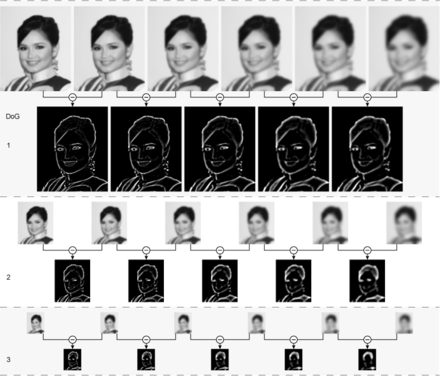
\includegraphics[scale=0.75]{DoG.png}
    \caption{Difference of Gaussians illustration (example from wikipedia)}\label{fig:Difference of Gaussians}
\end{figure}
After doing that, the algorithm must discriminate and precise the coordinate of a part of the key-point. Indeed, using different resolutions give some imprecise coordinate so it's necessary to make an interpolation to obtain the coordinate corresponding to the original image for key-point extracted from the most reduced resolutions images.  It is necessary to remove some kind of point too. The points that have not enough contrast comparing to the other are removed as the points that are on ridges (these points are really unstable and could move or disappear for many reasons so it's better to remove them).

When these operations have been computed, we obtain a set of key-points that characterize the image. This method allows to obtain the key-points to characterize an image without taking a predefined set of point. So the set of points obtained is potentially lighter than the one obtained by the dense grid method and it is more accurate because only important points wherever they are are conserved.


\subsubsection{Dense Grid}
The dense grid method is the easiest way to extract key-points.
The image has first to be divided into k sub-images and the intersections of the sub-images' outlines become the key-points.

\begin{figure}[h]
    \center
    \includegraphics[scale=1]{Dense_grid.png}
    \caption{Dense grid}\label{fig:dense_grid}
\end{figure}

\subsection{Descriptors}
The detection of key-points in images is increasingly used because it helps to do many tasks for example recognition, images assembly, 3D modeling, image indexation, video tracking etc. The key-points extraction in one image allows characterizing this image. Comparing the key-points of two images we can deduce if they have common information or not.
\subsubsection{SIFT}
SIFT (scale-invariant feature transform) is an algorithm used in sector of computer vision for detection and identification of similar elements between different numeric images.
The principal method proposed by the author David Lowe is to calculate the SIFT descriptors on images studied. These descriptors are numeric information which derived of local analysis of the image and they characterize the visual content of this image so that this one is independent of the scale, the framing, the angle of observation and the luminosity.
\begin{itemize}
	\item Scale-space extrema detection: In this step the key-points detection is done in scale space with three dimensions: the Cartesian coordinates(x,y) and the scale factor $\sigma$. The Gradient with scale factor $\sigma$ is given by the following equation.
	
 $$L(x,y,k\sigma)= G(x,y,k\sigma)*I(x,y)$$

This convolution allows smoothing the original image in such a way that details which radius is smaller than $\sigma$ value are stomped. The detection of objects which dimensions are approximately equal to $\sigma$ is done by the difference of Gaussion (DoG).
 $$D(x,y,\sigma)=L(x,y,k_i\sigma)-L(x,y,k_j\sigma)$$
Where k is the fixed factor of the algorithm and depends to the finesse of the scale space.
	\item Orientation assignment: On the base of local image gradient detections each key-point detected is assigned to one or many orientations. Insofar as descriptors are calculated from these orientations, it is important to safeguard the invariance of these descriptors to the rotation because whatever the orientation we must obtain the same descriptors using the same image.

For example with a key-point ($x_0$,$y_0$,$\sigma_0$), the calculation is done on the Gradient of the pyramid L(x,y,$\sigma_0$) which factor is nearest the scale factor of the point. In this way the calculation is also independent to the scale variance. With the symmetric finite difference, the gradient and the amplitude are calculated for each position around the key-point.
The calculation of these two factors is given by the following relations:
$$m(x,y)=\sqrt{(L(x+1,y)-L(x-1,y))^2+(L(x,y+1)-L(x,y-1))^2}$$
$$\theta(x,y)=atan2(L(x,y+1)-L(x,y-1),L(x+1,y)-L(x-1,y))$$
A histogram with 36 intervals is realized on the vicinity and each interval covering an angle of 10 degrees. On one hand, the histogram is moderated by a Gaussian window circular with a factor equal to 1.5 times of the scale factor of the key-point . On the other hand by the amplitude of each point. The peaks in this histogram correspond to the dominant orientations. All dominant orientations allow to have at least 80\% of the maximum value are taking in consideration and other additional key-points are detected. These new key-points detected are only different by the principal orientation.

	\item Key-point descriptor:Key-point descriptor: In this stage, a descriptor vector is created for each key-point detected such the descriptor is distinctive and invariant to the remaining variations like illumination, 3D viewing, etc. This stage is made on image which is more near the scale of the key-point scale.

The local system coordinates is modified for guarantee the invariance to the rotation by using an angle rotation equal to the orientation of the key-point in reverse direction.  Then, an area of 16x16 pixels is taken around the key-point; subdivide in 4x4 zones of 4x4 pixels each one. A histogram including 8 intervals is calculated on each zone. At each point of the zone, the orientation and the amplitude are calculated like previously. The orientation determines the interval to increment in the histogram which done by double weighted by the amplitude and by a center window Gaussian on the key-point of parameter 1.5 times of the scale factor of the key-point.

After that, the 16 histograms with 8 intervals each one, are concatenated and normalized. In object to reduce the sensibility of the descriptor to the changes of the luminosity, the values are fixed to 0.2 and the histogram is calculated again for finally give the descriptor of the key-point of 128 dimension.



\end{itemize}


\subsubsection{SURF}

In computer vision, Speeded Up Robust Features (SURF) is a local feature detector that can be used for tasks such as object recognition or 3D reconstruction. It is partly inspired by the scale-invariant feature transform (SIFT) descriptor. The standard version of SURF is several times faster than SIFT and claimed by its authors to be more robust against different image transformations than SIFT.

SURF uses an integer approximation of the determinant of Hessian blob detector, which can be computed with 3 integer operations using an integral image. For features, it uses the sum of the Haar wavelet response around the point of interest. These can also be computed with the aid of the integral image.

SURF descriptors can be used to locate and recognize objects, people or faces, make 3D scenes, track objects and extract points of interest.

SURF was first presented by Herbert Bay et al. at the 2006 European Conference on Computer Vision. An application of the algorithm is patented in the US.
\subsubsection{SIFT vs SURF}
The recognition of images or objects, is one of the most important applications of computer vision, becomes a comparison of local descriptors SIFT (Scale Invariant Feature Transform) and SURF (Speeded-UP Feature transform). These two local descriptors detect structures or very significant points in an image for a discriminating description of these areas from its neighboring points, in order to compare them with other descriptors using similar measures.
	
	
		

\subsubsection{Opponent SIFT}

The opponent SIFT descriptor is an algorithm using the same method as the standard SIFT descriptor except for the fact that it calculates three descriptors for each Key-points, obtained from the color opponent channel and defined as

\begin{equation}
O_{1} = \frac{R - G}{\sqrt{2}}, O_{2} = \frac{R + G - 2B}{\sqrt{6}}, O_{3} = \frac{R + G + B}{\sqrt{3}}.
\end{equation}

The opponent SIFT describes the three opponent color spaces : the two first channels $O_1$, $O_2$ contain some intensity information, but they are sensible to changes in light intensity. The last channel will contain the intensity information.

The strength of this method is that it uses a color space, and we can see directly information of that with the algorithm of the SIFT descriptor. The weakness is that the color space used is the RGB one.

\subsubsection{C$_2$O}

C$_2$O feature is a color descriptor which aim is to characterize an image by its color and texture characteristics. Indeed, the descriptors previously presented are satisfying to characterize images in gray or color levels but are pretty weak for highly textured images like nature pictures.
That's why the university of Poitiers has worked on a descriptor named C$_2$O (Color Contrast Occurrence), based on a vector including texture and color informations separately.
To compute it, there is two steps to follow : the calculation of the Color Contrast Occurrence Matrix and the feature (descriptor) from the matrix.



\paragraph{The Color Contrast Occurrence Matrix}
~~\\
~~\\
To compute this descriptor, the aim is to calculate a matrix which represents each key-point by a probability.
To compute it, the image has to be used in a color space which is able to separate best the color and the luminance information. Tests have shown that the CIE L* a* b* space separate "has minimum correlation between luminance and chrominance information" ("Color Contrast Occurrence, a full vector for color and texture").
So the image is passed in the CIE L* a* b* color space before the calculation of the descriptor.
Before the calculation of the L* a* b* space, its needed to transform our image through the XYZ space that is a perceptual space based on a linear transformation of the RGB space.


\vspace{0.5cm}
$$A=\begin{pmatrix}
	X_r&X_g&X_b\\
	Y_r&Y_g&Y_b\\
    Z_r&Z_g&Z_b
\end{pmatrix}$$
\vspace{0.5cm}
\begin{equation}
\begin{pmatrix}X\\Y\\Z\end{pmatrix}=A*\begin{pmatrix}R\\G\\B\end{pmatrix}
\end{equation}

With A a matrix which coefficients are depending on the chosen standard illuminant.
When this XYZ space has been computed, we have to compute the following transformation to get our image in the L* a* b* space.

\vspace{0.5cm}
\begin{equation}
L^*=  \left \{
   \begin{array}{l}
      116*(\frac{Y}{Y_0})^\frac{1}{3}-16~~~~si \frac{Y}{Y_0}>0.008856\\
   903.3*(\frac{Y}{Y_0})~~~~~~~~~~si \frac{Y}{Y_0}<0.008856\\
   \end{array}
   \right .
\end{equation}
\vspace{0.5cm}
\begin{equation}
a^*=500*\begin{bmatrix}f(\frac{X}{X_0})-f(\frac{Y}{Y_0})\end{bmatrix}
\end{equation}
\vspace{0.5cm}
\begin{equation}
b^*=300*\begin{bmatrix}f(\frac{Y}{Y_0})-f(\frac{Z}{Z_0})\end{bmatrix}
\end{equation}
After that, we can calculate the descriptor. The principle is simple : for each key-point, we have to calculate the probability to have a specific color difference between two pixels separated by a spatial vector (a voir si le dit vecteur est vecteur type). The color difference is calculated by considering the angles created by the L* a* b* representation and a perceptual distance (probablement sur la luminance mais a v�rifier).


So we define the color contrast occurrence value as : $\overrightarrow{\Lambda(C_i,C_j)}$
\begin{equation}
\overrightarrow{\Lambda(C_i,C_j)} : prob(\overrightarrow{\Lambda(C_i,C_j)} = \overrightarrow{\Lambda_\chi}
\end{equation}
\begin{equation}
~~~~~~~~~~~~~~~~~~~~ with~ \|\overrightarrow{\Lambda(C_i,C_j)}\| = \Delta E_\chi
\end{equation}
\begin{equation}
~~~~~~~~~~~~~~~~~~~~~~~~~~ and ~ \,(\overrightarrow{Oa},\overrightarrow{c_ic_j}) = (\alpha,\beta) = \,\overrightarrow{\Lambda_\chi}
\end{equation}

This computation gives us a cloud of point which characterizes the key-point by its color and texture neighborhood (see below).

\begin{figure}[h]
    \center
    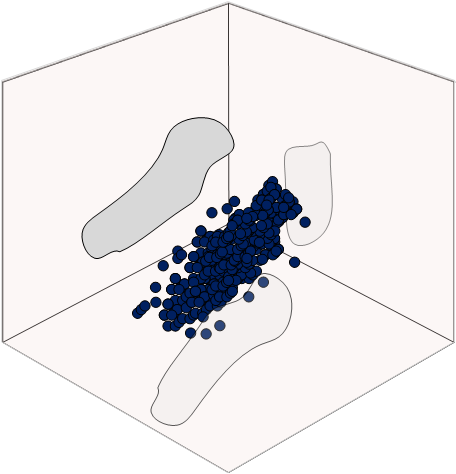
\includegraphics[scale=0.45]{IllustrationMatriceC2O.png}
    \caption{Color Contrast Occurrence Matrix}\label{fig:Color Contrast Occurence Matrix}
\end{figure}

On the figure shown above, we can see an example of the cloud of points that we expect to obtain. There are two thing which characterize the image :
\begin{itemize}
\item the size and the form of the cloud characterizing the texture around the key-point.
\item the projections on the three plans of the representation which characterize the color information around the key-point.
\end{itemize}
\paragraph{The Color Contrast Occurrence feature}
~~\\
~~\\
With the cloud of point obtained by the computation of the Color Contrast Occurrence matrix, we have a 3 dimensional representation of our key-point. To reduce the quantity of data to store and to facilitate the distance calculation, we have to represent this matrix by at least a 2-dimensional feature.
To do that, the solution used is to realize a spherical quantization on the cloud of point to have a histogram which will represent our key-point on two dimensions.
Mathematically, this quantization is expressed as follows :

\begin{equation}
Sig_{C_2O}(I) = h_{\Delta i\alpha j\beta k)} = prob(\Delta_i\leq\|\overrightarrow{\Lambda(C_i,C_j)}\|<\Delta_j+\Delta E_{step})
\end{equation}

\begin{equation}
~~~~~~~~~~~~~~~ and~  \frac{2\pi}{n_{\alpha}}j \leq \alpha < \frac{2\pi}{n_{\alpha}}(j+1)
\end{equation}
\begin{equation}
~~~~~~ and~ 0 \leq \beta < \frac{2\pi}{n_{\beta}}(k)
\end{equation}

Each sphere will include a number of points of the cloud, but to have a better distribution, each sphere will be split in some part as shown below :

\begin{figure}[h]
    \center
    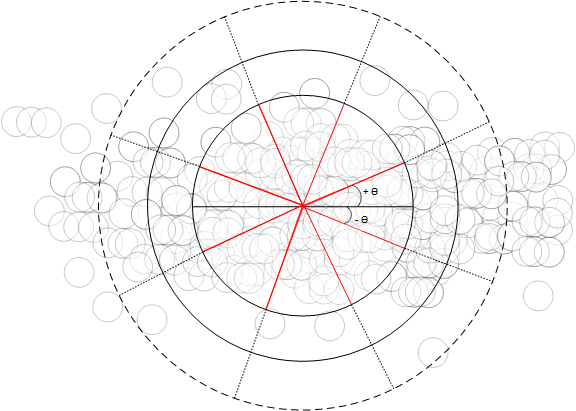
\includegraphics[scale=0.75]{QuantificationSpherique.png}
    \caption{Spheric quantizaton}\label{fig:Qantification sph�rique}
\end{figure}



Here we can see a sectional view of our spherical quantization. Each sphere is divided by n parts as shown above, and the number of points in each part are concatenated one by one in the description vector (quarter after quarter and sphere after sphere).
% ----------------------------------------------------------------
\end{document}